\section{Phong Illumination}
Illumination modeling is an important part of realistic rendering. It makes
colors more realistic, and enhances the perception of perspective in the final
image.
We will consider three kinds of lighting; ambient, diffuse, and specular.

\subsection{Ambient lighting}
Ambient lighting is the odd one out here. As a fixed-intensity, fixed-color
light that applies to all everything in the model, it corresponds to a
positionless (or omni-present) light source. It has no real-world pendant, but
provides a basic intensity value for all objects. Its only variable is the
object material, denoted $K_{a}(x)$. The ambient light value for a point $x$ is
found by the formula $$I_{ambient}(x) = I_{a}K_{a}(x)$$ Where $I_{a}$
represents the 'light source' intensity, and $K_{a}(x)$ an intensity weight for
the object material at the point $x$.

\subsection{Diffuse lighting}
When calculating the diffuse lighting in a single point in the phong shading
process, we estimate that the intensity of the light that is reflected does not
vary depending on the position from which the point is viewed. This is also
referred to as a lambertian reflectance. As our light source is of the type
'point' we use the following formula to calculate the reflection of light in a
single point on the surface:

$$I_{diffuse}(x) = Li(x) Kd(x) max(n(x) · l(x), 0)$$ $Li$ is the intensity of
the light source. The light intensity decreases as we move farther away from
the source. This is calculated through $Idiffuse(x) = Il(x) kd(x) max(n(x) ·
l(x), 0)$ In our model we assume that the light intensity does not decrease.
$Kd$ is the properties of the Lambertian surface. As some surfaces reflects
light more than others (ranging from perfect mirrors to total absorption of the
light), this property dictates how much of the light is reflected.

The $max(n(x) · l(x), 0)$ part finds the dot product between the light vector
and the normal in the point. If this value is less than zero, the angle between
the two is large enough for the light source to be behind the surface. As a
result the lighting value is set to zero (as all previous values are multiplied
by this factor). This makes sense, as as surface lit from behind would not
receive any direct illumination. The technique used is similar to the one used
in back face culling, where we also measure the normal. The difference between
the two being that in culling we used the vector from the camera to the
surface, and here we use the vector from the light source to the surface-point. 


\subsection{Specular lighting}
The specular lighting element uses the angles between a surface's normal $\vec{N}$
and the direction to the light source $\vec{l}$, and to the point of view $\vec{V}$
respectively, to determine an intensity weight based the amount of light reflected in
the direction of the viewer. Intuitively, the result should be inversely
proportional to $\alpha$.

The specular element is found by
$$I_{specular} = I_{s}K_{s}(\vec{R}\cdot\vec{V})^e$$
where $\vec{R}$ is $\vec{l}$ mirrored around $\vec{N}$, and $e$ is a measure of
the specularity sharpness.

\begin{figure}[hbtp]
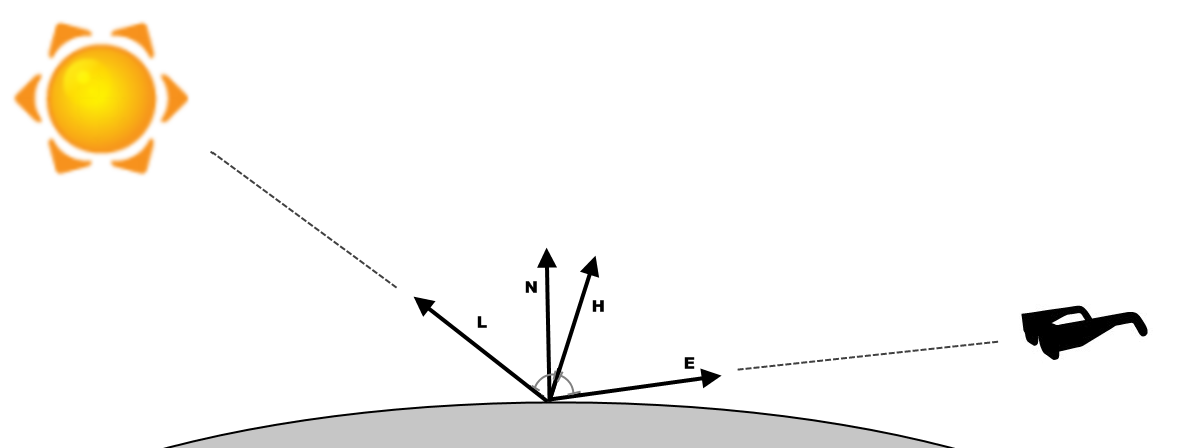
\includegraphics{pics/specularAngle.png}
\caption{}
\label{fig:specAng}
\end{figure}


When calculating the diffuse lighting in a single point in the phong shading process, we estimate that the intensity of the light that is reflected does not vary depending on the position from which the point is viewed.  This is also referred to as a lambertian reflectance. 
As our light source is of the type 'point' we use the following formula to calculate the reflection of light in a single point on the surface:

$$Idiffuse(x) = Li(x) Kd(x) max(n(x) · l(x), 0)$$
$Li$ is the intensity of the light source. The light intensity decreases as we move farther away from the source. This is calculated through 
$Idiffuse(x) = Il(x) kd(x) max(n(x) · l(x), 0)$
In our model we assume that the light intensity does not decrease.
$Kd$ is the properties of the Lambertian surface. As some surfaces reflects light more than others (ranging from perfect mirrors to total absorption of the light), this property dictates how much of the light is reflected.

The $max(n(x) · l(x), 0)$ part finds the dot product between the light vector and the normal in the point. If this value is less than zero, the angle between the two is large enough for the light source to be behind the surface. As a result the lighting value is set to zero (as all previous values are multiplied by this factor). This makes sense, as as surface lit from behind would not receive any direct illumination. The technique used is similar to the one used in back face culling, where we also measure the normal. The difference between the two being that in culling we used the vector from the camera to the surface, and here we use the vector from the light source to the surface-point. 


\subsection{Specular lighting}
The specular lighting element uses the angles between a surface's normal $\vec{N}$
and the direction to the light source $\vec{l}$, and to the point of view $\vec{V}$
respectively, to determine an intensity weight based the amount of light reflected in
the direction of the viewer. Intuitively, the result should be inversely
proportional to $\alpha$.

The specular element is found by
$$I_{specular} = I_{s}K_{s}(\vec{R}\cdot\vec{V})^e$$
where $\vec{R}$ is $\vec{l}$ mirrored around $\vec{N}$, and $e$ is a measure of
the specularity sharpness.

\begin{figure}[hbtp]
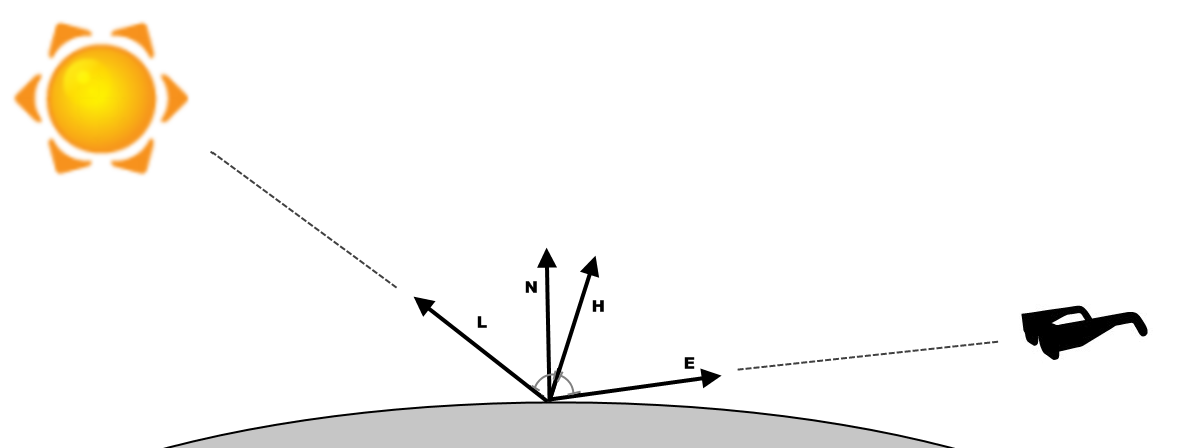
\includegraphics{pics/specularAngle.png}
\caption{}
\label{fig:specAng}
\end{figure}

